\documentclass[../cond-mat-theory.tex]{subfiles}
\pagebreak
\section{Problems from Ashcroft / Mermin}

\subsection{Poisson Distribution}
In the Drude model, the probability of an electron suffering a collision in an infinitesimal time $dt$ is $dt/\tau$.

\subsubsection{Probability of no collision}\label{qn:01-1a} \textit{Show that an electron picked at random at a given moment had no collision during the preceding t seconds with probability} $\euler^{-t/\tau}$. \textit{Show that it will have no collision during the next t seconds with the same probability.}

\begin{multicols}{2}
We need to derive that the process is actually a Poisson distribution.
Consequently, we know that in a very small time the probability of a collision is $dt/\tau$. The probability of avoiding a collision is then:
\begin{align}
	\rho_{\text{avoid}} = 1 - \frac{dt}{\tau}
\end{align}
If we have some time t, we can break it up into N parts, and let N approach infinity to satisfy the infinitesimal quantity.
\begin{align}
	\frac{t}{N} = \Delta t, \lim\limits_{N \to \infty}\left(\Delta t\right) = dt
\end{align}
By multiplying the probability of avoiding collision with N segments of infinitesimal time together, we get:
\begin{align}
	\rho_{\text{avoid}}(t) &= \left(1-\frac{\Delta t}{\tau}\right)^N = \left(1-\frac{t}{N\tau}\right)^N
\end{align}
Here we can use a limit theorem, 
\begin{align}
\lim\limits_{x\to\infty}\left(1 + \frac{a}{x}\right)^x = \euler^a
\end{align}
and so we have
\begin{align}
	\lim\limits_{N\to\infty}\rho_{\text{avoid}}(t) = \euler^{-t/\tau}
\end{align}
\end{multicols}

\subsubsection{Probability of collision in small interval}\label{qn:01-1b} \textit{Show that the probability that the time interval between two successive collisions of an electron falling in the range between t and t+dt is} $(dt/\tau)\euler^{-t/\tau}$.

\begin{multicols}{2}
	We already have the probability of not colliding by time $t$. The probability of a collisions after infinitesimal time dt is given from the introduction $dt/\tau$. Therefore the probability of colliding at some time small interval of time is given by:
	\begin{align}
		\rho_{t\to t+dt} &= \rho_{\text{avoid}}(t) \times \rho_{\text{collide}}\left(dt\right)\\
		&= \euler^{-t/\tau} \left(\frac{dt}{\tau}\right)
	\end{align}
	Note it may be tempting to calculate the probability of colliding within an interval as 
	\begin{align}
		1 - \frac{1}{\tau}\int_t^{t+dt}\euler^{-t'/\tau}dt'
	\end{align}
	but note that this includes multiple new collisions, not just a single collision. 
\end{multicols}

\subsubsection{Mean time to next collision / previous collision using a)}\label{qn:01-1c}\textit{ Show that as a consequence of (a) that at any moment the mean time back to the last collision (or up to the next collision) averaged over all electrons is} $\tau$.
\begin{multicols}{2}
	The expectation value of a probability distribution function (PDF) for x is given by the integral:
	\begin{align}
		\text{Exp}(x) = \int_0^\infty x \times \text{PDF}(x)dx
	\end{align}
	We have already found the PDF in part \cref{qn:01-1a}, but need to multiply a normalisation factor $\frac{1}{\tau}$.
	Using the integration by parts, $x \euler^{-ax}dx = -\frac{x}{a}\euler^{-ax} + \frac{1}{a}\euler^{-ax}dx$, we can evaluate the integral:
	\begin{align}
		\braket{t} &= \frac{1}{\tau}\int_{0}^{\infty} t \euler^{-t/\tau} \\
		&= \frac{1}{\tau}\left[-\left(t\tau\right)^{-t/\tau}\right]_{0}^{\infty} + \frac{1}{\tau}\int_{0}^{\infty}\tau \euler^{-t/\tau}dt\\
		&= 0 + \left[-\tau \euler^{-t/\tau}\right]_{0}^{\infty} = \tau
	\end{align}
\end{multicols}

\subsubsection{Mean time between collisions using b)}\label{qn:01-1d} \textit{Show as a consequence of (b) that the mean time between successive collisions of an electron is} $\tau$.\\

\textcolor{red}{This question seems a little redundant and I'm not quite sure what the purpose of it is.}%TODO Remove

\begin{multicols}{2}
	In \cref{qn:01-1b} we found the probability of no collisions then a collision is:
	\begin{align}
		p_{t\to t+dt} = \euler^{-t/\tau}\left(\frac{dt}{\tau}\right)
	\end{align}
	Using this result, we can find the average time as:
	\begin{align}
		\braket{t} = \int_{0}^{\infty} t \euler^{-t/\tau}\left(\frac{1}{\tau}\right)dt
	\end{align}
	However this is the same integral as in \cref{qn:01-1c}, so the result is the same. 
\end{multicols}

\subsubsection{Drude's mistakes}\label{qn:01-1e}
\textit{Part (c) implies that any moment the time T between the last and next collision averaged over all electrons is} $2\tau.$ \textit{Explain why this is not inconsistent with the result in (d) (A thorough explaination should include a derivation of the probability distribution for T). A failure to appreciate this subtlety led Drude to a conductivity only half of (Eq1.6, Ashcroft \& Mermin). He did not make the same mistake in the thermal conductivity, whence the factor of two in his calculation of the Lorenz number.}

\begin{multicols}{2}	
	To deriving the probability distribution for T, we need to recognise it's the join distribution of two distributions, which implies convolving the two links between the time to the previous and the time to the next, consequentially integrate over a intermediate time $t_1$.
\end{multicols}
\begin{multicols}{2}
	\begin{align}
		P(T) &= \int_{0}^{T}\euler^{-(T-t_1)/\tau}\left(\frac{1}{\tau}\right) \times \euler^{-t_1/\tau}\left(\frac{dt_1}{\tau}\right)\\
		&= \int_{0}^{T} \euler^{-T/\tau}\left(\frac{1}{\tau^2}\right)dt_1\\
		&= \frac{T\euler^{-T/\tau}}{\tau^2}
	\end{align}
	
	The expectation of such a distribution is as follows:
	\begin{align}
	\braket{T} &= \int_{0}^{\infty} T P(T) dT\\
	&=\int_{0}^{\infty} T \frac{T\euler^{-T/\tau}}{\tau^2}dT\\
	&=\left[-\tau \frac{T^2}{\tau^2}\euler^{-T/\tau}\right]_{0}^{\infty} + 2\int_{0}^{\infty} \frac{T\euler^{-T/\tau}}{\tau}dT\\
	&\nonumber\text{First bounded term disappears,}\\
	&\nonumber\text{substitute } T = -\tau \log(u), dT = -\tau \frac{1}{u} du\\
	&= 0 + 2 \int_{1}^{0} \frac{T}{\tau}u \times \frac{-\tau}{u} du\\
	&= 2\int_{0}^{1}Tdu = -2\tau\int_{0}^{1} \log (u) du\\
	&= -2\tau\left[-u+u\log (u)\right]_{0}^{1} = 2\tau
	\end{align}
	The result above is as expected. 
	
	The result is not inconsistent with (d) because the probability from \textit{any} time to the next collisions is always the same. Therefore it is a result of choosing the initial condition of being from a collisions that has just occurred, or in between two collisions, where no collision has occurred. Because Poisson like distributions don't keep track of past events, the expectation time till the next collision is always same no matter the initial condition.
	
\end{multicols}

\subsection{Joule Heating}
Consider a metal at a uniform temperature in a static uniform electric field \textbf{E}. An electron experiences collision, and then, after a time \textit{t}, a second collision. In the Drude model, energy is not observed in collisions, for the mean speed of an electron emerging from a collision does not depend on the energy that the electron acquired from the field since the time of the preceding collision. 

\subsubsection{Average energy loss}\label{qn:01-2a} \textit{Show that the average energy lost to the ions in the second of two collisions separated by a time } $t$ \textit{is} $(eEt)^2/2m$. \textit{(The average is over all directions in which the electron emerged from the first collision)}

\begin{multicols}{2}
	If the time between collisions is t, then the acceleration on the object is
	\begin{align}
		\mathbf{a_E} = \frac{-e \mathbf{E}}{m_e}
	\end{align}
	Calculating gained velocity:
	\begin{align}
		\Delta v &= \int_{0}^{t} \mathbf{a_E}dt\\
		&= \frac{-e\mathbf{E}t}{m_e}
	\end{align}
	Calculating the kinetic energy: 
	\begin{align}
		\delta E_k &= \frac{1}{2} m_e \left(\frac{-e\mathbf{E}t}{m_e}\right)^2\\
		&= \frac{\left(e\mathbf{E}t\right)^2}{2m_e}
	\end{align}
\end{multicols}

\subsubsection{Average energy loss from Q1}\label{qn:01-2b} \textit{Show using the result of \cref{qn:01-1b} that the average energy loss to the ions per electron per collision is} $(e\mathbf{E}\tau)^2/m$\textit{, and hence that the average loss per cubic centimeter per second is } $(n\euler^2\tau/m)\mathbf{E}^2=\sigma \mathbf{E^2}$. \textit{Deduce that the power loss in a wire of length L and cross section A is} $I^2R$, \textit{where I is the current flowing, and R is the resistance.}
\begin{multicols}{2}
	We know from Drude theory that the DC conductivity of a metal under the influence of an electric field can be calculated from the net acceleration each particle experiences before a collision. Using the averaged collision time $\tau$ this gives an average velocity and in turn a net conductivity:
	\begin{align}
	j &= -n e v\\
	v_{avg} &= \frac{v_f - v_i}{2}=\left(\frac{-\euler E}{m_e}\tau - 0\right)/2\\
	\implies j &= -\frac{n\euler^2\tau}{2m_e}E\\
	\sigma &= \frac{n\euler^2\tau}{2m}
	\end{align}
	
	From question 1, we have the probability of two successive collisions falling between t and t+dt is $(dt/\tau)\euler^{-t/\tau}$. 
	
	\textcolor{red}{Figure out how to generate same result but using Q1? Unclear.}
	
	To calculate the loss per cubic centimetre, recognise there are $n$ conduction electrons per cubic centimetre, and these on average collide every $\tau$ seconds. Then the energy loss is per cubic centimetre per second is:
	\begin{align}
		\frac{dE}{dt} = n\times \Delta E / \tau = \frac{n\euler^2\tau}{m}E^2 = \sigma E^2
	\end{align}
	Following this, we know that in a wire with cross section A and length L, that there will be a power loss of
	\begin{align}
		P &= L \times A \times \frac{dE}{dt}\\
		&= AL \times \frac{n\euler^2\tau}{m}E^2 = AL \times \sigma E^2 \label{eqn:01-2bp}
	\end{align}
	Note that adding in dimensional factors to ohms law gives:
	\begin{align}
		{V} &= R {I}\\
		\left(\frac{{V}}{L}\right) &= \left(\frac{A}{L}R\right) \left(\frac{{I}}{A}\right)\\
		{E}  &=\frac{1}{\sigma}{J}
	\end{align}
	Recognising the same terms in \cref{eqn:01-2bp}, we then have:
	\begin{align}
		P &= AL\times \sigma E^2 \\	
		&= \frac{A^2L}{A} \frac{\sigma^2}{\sigma} E^2 \\
		&= \left(A j\right)^2 \left(\frac{L}{A}\frac{1}{\sigma} \right) = I^2 R
	\end{align}
	
\end{multicols}

\subsection{Thomson Effect} \label{qn:01-3}
\textit{Suppose that in addition to the applied electric field in Problem 2 there is also a uniform temperature gradient} $\nabla T$ \textit{in the metal. Since an electron emerges from a collision at an energy determined by the local temperature, the energy lost in collisions will depend on how far down the temperature gradient the electron travels between collisions, as well as on how much energy it has gained form the electric field. Consequently the power lost will contain a term proportional to} $\mathbf{E}\cdot \nabla T$ \textit{(which is easily isolated from the other terms since it is the only term in the second-order energy loss that changes sign when the sign of }$\mathbf{E}$\textit{ is reversed). Show that this contribution in the Drude model by a term of order} $(ne\tau/m) (d\mathcal{E}/dT)(\mathbf{E}\cdot\nabla T)$, \textit{where} $\mathcal{E}$ \textit{is the mean thermal energy per electron. (Calculate the energy lost by a typical electron collision at} $\mathbf{r}$, \textit{which made its last collision at} $\mathbf{r-d}$). \textit{Assuming a fixed, energy-independent relaxation time $\tau$, \textbf{d} can be found to be linear in order in the field and temperature gradient by simple kinematic arguments which is enough to give the energy loss to second order.)}

\begin{multicols}{2}
	To show the additional term, consider the energy lost over some temperature gradient via the Drude model. In the original Drude model, we had particles colliding at some uniform temperature, scattering with a new velocity/direction proportional to the temperature. This temperature now has a gradient.
	
	Say the electron starts at some position with temperature / energy $\mathcal{E}_i$ and moves through temperature to a new temperature corresponding to energy $\mathcal{E}_f$. On average without an electric field, velocity is random and so energy is gained or lost in equal amounts as the particle "collides" according to the Drude model either side of the gradient. 
	
	However, in the presence of an electric field, the average velocity is non-zero, and so there is a net movement of thermal energy, which depends on the dot product of the electric field and the uniform temperature gradient. 
	
	Repeating the calculation from Q2 for the average velocity gained in collision time $\tau$ we have
	\begin{align}
		\mathbf{v} &= \int_{0}^{\tau} \frac{-e \mathbf{E}}{m_e}dt \\
		&= -\frac{e\mathbf{E}\tau}{m_e}
	\end{align}
	We do not need to find the distance travelled before a second collision, because it's rather the rate of motion across temperature, across a change in the thermal energy of electrons, that implies a loss of energy per unit time.
	%	CALUCLATION FOR DISTANCE D.
	%	\begin{align} 
	%		\mathbf{d} &= \int_{0}^{\tau} -\frac{e\mathbf{E}t}{m_e}dt\\
	%		&= \frac{-e\mathbf{E}\tau^2}{2m_e}
	%	\end{align}
	
	Therefore considering the power loss of a single electron, it's velocity determines how far it moves across a temperature gradient $\nabla_d T$ through space, which in turn determines how much the thermal energy $\mathcal{E}$ of the particle will change.
	\begin{align}
		\nabla P &= \mathbf{v} \cdot \mathbf{\nabla}T \times \frac{d\mathcal{E}}{dT} \\
		&= \frac{-e\mathbf{E}\tau}{m_e}\cdot \mathbf{\nabla}T \times \frac{d\mathcal{E}}{dT}\\
		&=  \frac{-e\tau}{m_e}\left(\frac{d\mathcal{E}}{dT}\right)\left(\mathbf{E}\cdot\mathbf{\nabla}T\right) 
	\end{align}
	It is simple to add in the factor n, which is the number of electrons.
\end{multicols}

\subsection{Helicon Waves}
\textit{Suppose that a metal is placed in a uniform magnetic field } \textbf{H} \textit{along the z-axis. Let an AC electric field } $\mathbf{E}\euler^{-\imag\omega t}$ \textit{be applied perpendicular to }\textbf{H}.
\subsubsection{Circular polarisation}
\textit{If the electric field is circularly polarized ($E_y=\pm iE_x$) show that Eq. (1.28) must be generalised to }
\begin{align}
	j_x = \left(\frac{\sigma_0}{1-\imag(\omega \mp \omega_c)\tau}\right)E_x
\end{align}
\begin{multicols}{2}
	\paragraph{Attempt at dynamic solution}
		If the momentum of the electrons is influenced by an AC electric field and a constant magnetic field, we can consider the new equation of motion for the electrons.
		\begin{align}
			\frac{d\mathbf{p}}{dt} = -e\mathbf{E} -\frac{e\mathbf{p}}{m_ec}\times\mathbf{H} - \frac{\mathbf{p}}{\tau}
		\end{align}
		Note that the last term comes from the infinitesimal probability of considering electrons that don't crash (ie, $1-\frac{dt}{\tau}$), and neglecting second order terms that contribute to the Lorentz force components.
		Here our electric field has the form
		\begin{align}
			\mathbf{E}(t) &= \begin{bmatrix}E_x\\E_y\end{bmatrix}\euler^{-\imag\omega t}\\
			&=\begin{bmatrix}E_x\\\pm \imag E_x\end{bmatrix}\euler^{-\imag\omega t}
		\end{align}
		Noting $\hat{y}\times\hat{z} = \hat{x}$ and $\hat{x}\times\hat{z}=-\hat{y}$ Calculating the components, where $\omega_c=\frac{eH_z}{m_ec}$ , we have
		\begin{align}
			\frac{dp_x}{dt} &= -\euler E_x \euler^{-\imag\omega t} - \omega_c p_y -\frac{p_x}{\tau}\\
			\frac{dp_y}{dt} &= -\euler E_y \euler^{-\imag\omega t} + \omega_c p_x -\frac{p_x}{\tau}
		\end{align}
		The dynamical solution for these simultaneous equations, solved through Mathematica is
		\begin{align}
		p_x(t) &= \frac{e\tau{E_y}}{\tau  {\omega_c} - 1}\euler^{-\imag t \omega}\\
		{p_y}(t) &= \frac{(e {E_x} - e{E_y} - e \tau  {\omega_c} {E_x})}{{\omega_c} (\tau  {\omega_c} - 1)}\euler^{-\imag t \omega }
		\end{align}
		Consequently, we can now multiply both sides by the factor $ne/m$ to convert the momentum of an electron to the current density. However, this doesn't yield the target equation, and so we instead need to look towards the steady state solution as demonstrated on page 16 of Ashcroft \& Mermin.
%		\begin{align}
%			\frac{nep_x(t)}{m} &= -\left(\frac{n\euler^2\tau}{m}\right)\frac{E_y \euler^{-\imagt\omega}}{\tau \omega_c + 1}\\
%			j_x(t)&= \mp i\left(\frac{\sigma_0}{\tau w_c + 1}\right)\left(E_x \euler^{\imag \omega t}\right)
%		\end{align}
	
	\paragraph{Attempt at steady state solution}
		Treat the electric field and the momentum as a time and frequency dependent component.
		\begin{align}
			E(t) = E(\omega)\euler^{-\imag\omega t}\\
			p(t) = p(\omega)\euler^{-\imag\omega t}
		\end{align}
		Then substituting into the same equation of motion, we have:
		\begin{align}
			-\imag \omega p_x(\omega) &= -\euler E_x(\omega) - \omega_c p_y -\frac{p_x}{\tau}\\
			-\imag \omega p_y(\omega) &= -\euler E_y(\omega) + \omega_c p_x -\frac{p_y}{\tau}
		\end{align}
		Rearranging:
		\begin{align}
			\left(-\imag\omega + \frac{1}{\tau}\right)p_x(\omega) = -\euler E_x(\omega) - \omega_c p_y(\omega)\\
			\left(-\imag\omega + \frac{1}{\tau}\right)p_y(\omega) = -\euler E_y(\omega) + \omega_c p_x(\omega)
		\end{align}
		
	\end{multicols}
		Solving the equations by substituting $p_y$,
		\begin{align}
			\left(-\imag\omega + \frac{1}{\tau}\right)p_x(\omega) &= -\euler E_x(\omega) - \omega_c  \frac{-\euler E_y(\omega) + \omega_c p_x(\omega)}{\left(-\imag\omega + \frac{1}{\tau}\right)}\\
			\left(-\imag\omega + \frac{1}{\tau} + \frac{\omega_c^2}{(-\imag \omega + \frac{1}{\tau})}\right)p_x(\omega) &= -\euler E_x(\omega) - \omega_c  \frac{-\euler E_y(\omega) }{\left(-\imag\omega + \frac{1}{\tau}\right)}\\
			\left(\left(-\imag\omega + \frac{1}{\tau}\right)\left(-\imag \omega + \frac{1}{\tau}\right) + {\omega_c^2}\right)p_x(\omega) &= \left(-\imag \omega + \frac{1}{\tau}\right)\left(-\euler E_x(\omega) - \omega_c  \frac{-\euler E_y(\omega) }{\left(-\imag\omega + \frac{1}{\tau}\right)}\right)\\
			\left(-\omega^2 - 2\imag\frac{\omega}{\tau} + \frac{1}{\tau^2}+ {\omega_c^2}\right)p_x(\omega) &= -\euler\left(-\imag \omega + \frac{1}{\tau}\right)E_x(\omega) + \euler\omega_c E_y(\omega)\\
			\left(-\omega^2 - 2\imag\frac{\omega}{\tau} + \frac{1}{\tau^2} + {\omega_c^2}\right)p_x(\omega) &= -\euler\left(-\imag \omega + \frac{1}{\tau} \mp \imag\omega_c\right)E_x(\omega)\\
			p_x(\omega) &= \frac{-\euler\left( 1 -  \imag \left(\omega  \mp\omega_c\right)\tau\right)}{\tau\left(-\omega^2 - 2\imag\frac{\omega}{\tau} + \frac{1}{\tau^2} + {\omega_c^2}\right)}E_x(\omega)
		\end{align}
		Note here that we can factor the denominator as such:
		\begin{align}
		\left(\omega_c^2 - \omega^2 - 2i\frac{\omega}{\tau} + \frac{1}{\tau^2}\right) &= \left(\frac{1}{\tau} - i\omega\right)^2 + \omega_c^2\\
		&= \left(\frac{1}{\tau} - \imag\omega + \imag\omega_c\right) \left(\frac{1}{\tau} - i\omega - \imag\omega_c\right)\\
		&= \frac{1}{\tau^2}\left(1 - \imag\left(\omega + \omega_c\right)\tau\right) \left(1 - \imag\left(\omega - \omega_c\right)\tau\right)\\
		&= \frac{1}{\tau^2}\left(1 - \imag\left(\omega \pm \omega_c\right)\tau\right) \left(1 - \imag\left(\omega \mp \omega_c\right)\tau\right)
		\end{align}
		Cancelling the common factors provides the result:
		\begin{align}
			p_x(\omega) &= \frac{-\euler\tau}{\left(1 - \imag\left(\omega \pm \omega_c\right)\tau\right)}E_x(\omega)
		\end{align}
		Multiplying by the factor $\frac{ne}{m_e}$ to get the current density, we have 
		\begin{align}
			j_x(\omega) = \left(\frac{n\euler^2\tau}{m_c}\right) \frac{1}{1-\imag(\omega\pm\omega_c)\tau}E_x(\omega)&\\
			= \frac{\sigma_0}{1-\imag(\omega\pm\omega_c)\tau}E_x(\omega)&
		\end{align}
		\textcolor{red}{Note the $\pm$ seems to be the wrong sign, but I can't find the sign error in this working.}
	
\subsubsection{Maxwell's equations soln}
\textit{Show that, in conjunction with (1.61), Maxwell's equation (1.31) have a solution}
\begin{align}
	E_x = E_0\euler^{i\left(kz-\omega t\right)}, E_y=\pm i E_x, E_z = 0
\end{align}
\textit{provided that} $k^2c^2=\epsilon \omega^2$ \textit{where} 
\begin{align}
	\epsilon(\omega) = 1 - \frac{\omega_p^2}{\omega}\left(\frac{1}{\omega \mp \omega_c + i/\tau}\right)
\end{align}\\

\begin{multicols}{2}
	\paragraph{Maxwell's Equations}
	Generally, in Gaussian units:
	\begin{align}
		\nabla \cdot \mathbf{E} = 4\pi \rho \\\nabla \cdot \mathbf{H} = 0\\
		\nabla \times \mathbf{E} = -\frac{1}{c}\frac{\partial \textbf{H}}{\partial t}\\
		\nabla \times \mathbf{H} = \frac{1}{c} \left(4\pi\mathbf{J} + \frac{\partial \textbf{E}}{\partial t}\right)
	\end{align}
	Because we're looking at metals, there are no bound charges. Therefore Maxwells equation's can be written as
	\begin{align}
		\nabla \cdot \mathbf{E} = 0\\\nabla \cdot \mathbf{H} = 0\\
		\nabla \times \mathbf{E} = -\frac{1}{c}\frac{\partial\mathbf{H}}{\partial t}\\
		\nabla \times \mathbf{H} = \frac{4\pi}{c}\mathbf{j} + \frac{1}{c}\frac{\partial \mathbf{E}}{\partial t}
	\end{align}
	
	Taking the curl of Faraday's law of induction, using the zero divergence property, and assuming solutions that have $\euler^{-\imag \omega t}$ time dependence, 
	\begin{align}
		\nabla\times\left(\nabla \times \mathbf{E}\right) &= \nabla\times\left(-\frac{1}{c}\frac{\partial \textbf{H}}{\partial t}\right)\\
		\nabla\left(\nabla \cdot \textbf{E} \right)-\nabla^2 \textbf{E} &= -\frac{1}{c} \left(\nabla \times \frac{\partial}{\partial t}\mathbf{H}\right)\\
		0 -\nabla^2 \textbf{E}  &= \frac{\imag\omega}{c} \left(\nabla \times \textbf{H}\right)\\
		\nabla^2 \textbf{E} &= - \frac{\imag\omega}{c} \left(\frac{4\pi}{c}\textbf{j} - \frac{\imag\omega}{c}\textbf{E} \right)
	\end{align}
	Using the result from the last part, we can write $\textbf{j}(\omega) = \sigma(\omega)\textbf{E}(\omega)$.
	\begin{align}
		\implies \nabla^2 \textbf{E} &= - \frac{\imag\omega}{c} \left(\frac{4\pi}{c}\sigma - \frac{\imag\omega}{c} \right)\textbf{E}\\
		&= -\frac{\omega^2}{c^2} \left(\frac{4\pi\imag\sigma}{\omega} + 1\right)\textbf{E}
	\end{align}
	
	Doing the same with the magnetic field yields:
	\begin{align}
		- \nabla^2 \mathbf{H} &= \frac{4\pi}{c}\nabla\times\mathbf{j} + \frac{\omega^2}{c^2} \mathbf{H}\\
		&= \frac{4\pi\sigma}{c} \left(-\frac{\imag\omega}{c}\mathbf{H}\right) +\frac{\omega^2}{c^2} \mathbf{H}\\
		&= \frac{\omega^2}{c^2}\left(1 - \frac{4\pi\sigma\imag}{\omega}\right)
	\end{align}
	
	Note, make sure to consider that the conductivity is a function of $\omega$, as shown in part a). 
	\begin{align}\label{eqn:01-maxwell}
		\implies\nabla^2 \textbf{E} &= -\frac{\omega^2}{c^2} \left(\frac{4\pi}{\omega}\frac{\sigma_0}{1-\imag(\omega\pm\omega_c)\tau}\imag + 1\right)\textbf{E}
	\end{align}
	
	\paragraph{Attempt 1 - Solving characteristic equation for solutions}
	We're looking for plane waves that propagate through a particular direction, in this case z. The solutions for the electric field then follow the general solutions of the wave equation:
	\begin{align}
		\textbf{E} = \textbf{E}_0\euler^{\lambda \textbf{z}}
	\end{align}
	Applying the 
	Solving coefficients:
	\begin{align}
		\lambda^2 &= -\frac{\omega^2}{c^2}\left(\frac{4\pi\sigma}{\omega}\imag + 1\right)\\
		\lambda &= \pm \imag \frac{\omega}{c} \sqrt{\frac{4\pi\sigma}{\omega}\imag + 1}
	\end{align}
	Let $z=a+b\imag$, and $z^2 = \frac{4\pi\sigma}{\omega}\imag + 1 = (a^2-b^2) + 2ab\imag$. Then equating the parts,
	\begin{align}
		a^2-b^2 &= 1\\
		2ab &= \frac{4\pi\sigma}{\omega}
	\end{align}
	Calculating a:
	\begin{align}
		\implies a^2 - \left(\frac{4\pi\sigma}{2\omega a}\right)^2 &= 1\\
		a^4 - a^2 - \left(\frac{2\pi\sigma}{\omega}\right)^2 &= 0\\
		\left(a^2 - \frac{1}{2}\right)^2 -\frac{1}{4} - \left(\frac{2\pi\sigma}{\omega}\right)^2 &= 0\\
		a^2 - \frac{1}{2} = \pm \sqrt{\frac{1}{4} + \left(\frac{2\pi\sigma}{\omega}\right)^2}&\\
		a = \pm \sqrt{\frac{1}{2} \pm \sqrt{\frac{1}{4} + \left(\frac{2\pi\sigma}{\omega}\right)^2}}
	\end{align}
	Calculating b:
	\begin{align}
		b&= \pm\sqrt{a^2 -1}\\
	 &= \pm\sqrt{-\frac{1}{2} \pm \sqrt{\frac{1}{4} + \left(\frac{2\pi\sigma}{\omega}\right)^2}}
	\end{align}
	Therefore, 
	
	\begin{align}
		E(x,t) &= E_0 \euler^{\imag\left(\lambda x-\omega t\right)}\\
		\lambda &= \pm \imag \frac{\omega}{c} \left(a +b\imag\right)
	\end{align}
	
	\paragraph{Attempt 2 - Verifying provided solution is valid}
		We have been provided with the solution:
		\begin{align}
			E_x = E_0 \euler^{\imag\left(kz-\omega t\right)},&& E_y = \pm \imag E_x,&& E_z=0
		\end{align}
%		with (\textcolor{red}{note, an erroneous term I believe? Corrected from $\omega_p^2$})
		\begin{align}
%			\epsilon(\omega) &= 1 - \frac{\textcolor{red}{\omega_p^1}}{\omega}\left(\frac{1}{\omega \mp \omega_c + i/\tau}\right)\label{eqn:01-epsilon}\\
			\epsilon(\omega) &= 1 - \frac{{\omega_p^2}}{\omega}\left(\frac{1}{\omega \mp \omega_c + i/\tau}\right)\label{eqn:01-epsilon}\\
			\omega_p^2&= \frac{4\pi n \euler^2}{m}\\
			\omega_c&= \frac{eH}{mc}\\
			k^2c^2 &= \epsilon\omega^2
		\end{align}
		Verifying this solution to the differential equation found above earlier,
		\begin{align}
			\nabla^2\textbf{E}&= \nabla^2 \left(\euler^{ikz-\omega t}\right)\mathbf{E_0}\\
			&= i^2 k^2 \textbf{E}\\
			&= - \frac{\omega^2}{c^2}\left
				(1 - \left(\frac{4\pi n \euler^2 }{m}\right) \frac{1}{\omega} \frac{1}{\omega \mp \omega_c + \imag / \tau}
			\right)\mathbf{E}\\ 
			&= - \frac{\omega^2}{c^2} \left(
			1 - \left(\frac{4\pi n \euler^2 }{m}\right) \frac{1}{\omega} \frac{-\tau\imag}{-i\left(\omega \mp \omega_c\right)\tau + 1}
			\right)\mathbf{E}\\ 
			&=- \frac{\omega^2}{c^2} \left(
			1 + \left(\frac{\tau n \euler^2 }{m}\right) \frac{4\pi}{\omega} \frac{1}{-i\left(\omega \mp \omega_c\right)\tau + 1}\imag
			\right)\mathbf{E}\\
			&=- \frac{\omega^2}{c^2} \left(
			1 + \frac{4\pi}{\omega} \frac{\sigma_0}{1-i\left(\omega \mp \omega_c\right)\tau}\imag
			\right)\mathbf{E}
		\end{align}
		which thus satisfies the result of Maxwell's equations in \cref{eqn:01-maxwell}.
		
\end{multicols}

\subsubsection{Sketch of $\epsilon$}
\textit{Sketch }$\epsilon(\omega)$ for $\omega>0$ \textit{(choosing the polarisation $E_y=iE_x$) and demonstrate that solutions to $k^2c^2=\epsilon\omega^2$ exist for arbitrary $k$ at frequencies $\omega > \omega_p$ and $\omega < \omega_c$. (Assume the high field condition $\omega_c\tau \gg 1$, and note that even for hundreds of kilogauss, $\omega_p/\omega_c\gg 1$.)}



\begin{multicols}{2}
	Plotting \cref{eqn:01-epsilon}:
\begin{figure}[H]
	\centering
	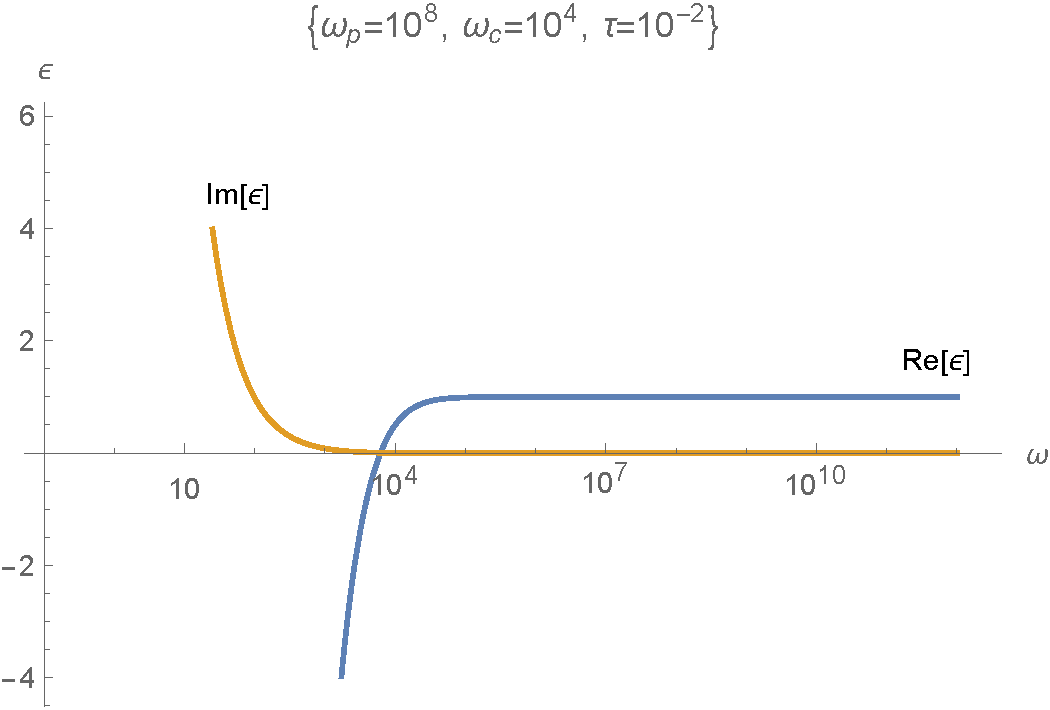
\includegraphics[width=0.9\linewidth]{a&m_01_4c}
\end{figure}	
Ideally the graph would demonstrate real solutions of $\epsilon$, which correspond to real wave-vectors $k$. However, if there are large imaginary components of $\epsilon$, then the wave solution has a large real exponential component, either suppressing or diverging based on sign. To demonstrate that real solutions, we first apply the assumptions to the function ($\omega_c \tau \gg 1, \omega_p/\omega_c\gg1$).
\begin{align}
	\epsilon(\omega) &= 1 - \frac{\omega_p^2}{\omega} \left(\frac{1}{\omega\mp \omega_c + i/\tau}\right)\\
	&=1 - \frac{\omega_p^2}{\omega \omega_c} \left(\frac{1}{\omega/\omega_c \mp 1 + \frac{i}{\tau\omega_c}}\right)\\
	&= 1 - \frac{\omega_p^2}{\omega \omega_c} \left(\frac{1}{\omega/\omega_c \mp 1 + 0}\right)\\
	&= 1 - \frac{\omega_p}{\omega} \left(\frac{1}{\omega/\omega_p \mp \omega_c/\omega_p}\right)\\
	&= 1 - \frac{\omega_p}{\omega} \left(\frac{1}{\omega/\omega_p \mp 0}\right)\\
	&= 1 - \frac{\omega_p^2}{\omega^2}
\end{align}

Therefore if $\omega > \omega_p$, then the clear implications are that the term $\frac{\omega_p}{\omega}$ approaches zero. Therefore $\epsilon(\omega)$ is real and positive, thereby resulting in a complex exponent and a propagating electromagnetic field.

If $\omega < \omega_c$, then we have to consider the limit that $\frac{\omega_p}{\omega_c}\gg 1$, which then implies $\frac{\omega_p}{\omega}\ggg 1$. In this case $\epsilon(\omega)$ is also real but negative, thereby also resulting in a complex exponent and a propagating electromagnetic field.
	
\end{multicols}

\subsubsection{Estimation of Helicon frequency}
\textit{Show that when $\omega \ll \omega_c$ the relation between $k$ and $\omega$ for the low-frequency solution is}
\begin{align}
	\omega = \omega_c \left(\frac{k^2c^2}{\omega_p^2}\right)
\end{align}
\textit{This low-frequency wave, known as a helicon, has been observed in many metals. Estimate the helicon frequency if the wavelength is 1cm and the field is 10 kilogauss, at typical metallic densities.}
\begin{multicols}{2}
	\paragraph{Low Frequency Solution}
	Starting with the condition from part b),
	\begin{align}
		\omega^2 \epsilon(\omega) &= k^2c^2\\
		\omega^2\left(1 - \frac{\omega_p^2}{\omega} \left(\frac{1}{\omega\mp \omega_c + i/\tau}\right)\right) &= k^2c^2 \\
%		\omega^2\left(1 - \frac{\omega_p^2}{\omega} \left(\frac{1/\omega_c}{\omega/\omega_c \mp \omega_c/\omega_c + i/(\tau\omega_c)}\right)\right) &= k^2c^2\\
%		\nonumber\text{Taking the limit }\omega\ll \omega_c&\\
%		\omega^2\left(1 - \frac{\omega_p^2}{\omega} \left(\frac{1/\omega_c}{\mp 1 + i/(\tau\omega_c)}\right)\right) &= k^2c^2\\
		\omega^2\left(1 - \omega_p^2\left(\frac{\frac{1}{\omega_c}}{\frac{\omega^2}{\omega_c} \mp \frac{\omega_c \omega }{\omega_c} + i\frac{\omega}{\tau\omega_c}}\right)\right) &= k^2c^2
	\end{align}
	When $\omega\ll \omega_c$,
	\begin{align}
		\omega^2\left(1 - \omega_p^2 \left(\frac{1/\omega_c}{\mp \omega}\right)\right) &= k^2c^2\\
		\nonumber \text{Assuming } \omega_p \gg \omega_c& \text{ as reasoned in part c).}\\
		\omega\left(\frac{\omega_p^2}{\omega_c}\right) &= k^2c^2\\
		\omega&=\omega_c \left(\frac{k^2c^2}{\omega_p^2}\right)
	\end{align}
	
	\paragraph{Estimation}
	\begin{align}
		\omega &= \omega_c \left(\frac{k^2c^2}{\omega_p^2}\right)\\
		\omega_p &= \frac{4\pi n \euler^2 }{m_e} \\
		\omega_c &= \frac{eH}{m_e c} 
	\end{align}
	Using typical free-electron metallic densities of $1\times10^{22}$ cm$^{-3}$, and inferring the wavevector $k = c/\lambda$, we get
	\begin{align}
		\omega = \frac{Hc}{2ne\lambda^2} = 308\text{ Hz}
	\end{align}
\end{multicols}

\subsection{Surface Plasmons}

\textit{An electromagnetic wave that can propogate along the suface of a metal complicates the observation of ordinary (bluk) plasmons. Let the metal be contained in the half space $z>0, z<0$ being vacuum. Assume that the electric charge density $\rho$ appearing in Maxwell's equations vanishes both inside and outside the metal. (This does not preclude a surface charge density concerntrated in the plane z=0.) The surface plasmon is a solution to Maxwell's equations of the form }

\begin{align}
	E_x = A\euler^{\imag q x - Kz} && E_y = 0, && E_z = B\euler^{\imag q x - Kz}, &&z>0;\\
	E_x = C\euler^{\imag q x - K'z} && E_y = 0, && E_z = D\euler^{\imag q x - K'z}, &&z<0;\\
	\left\{q,K,K'\right\}\in\mathds{R},&&\left\{K,K'\right\} > 0
\end{align}

\subsubsection{Relate q, K and K'}
\textit{Assuming the usual boundary conditions, (}$\mathbf{E_\parallel}$\textit{ continuous, }$(\epsilon \mathbf{E})_\perp$ \textit{continuous), and using the Drude results (1.35) and (1.29) find three equations relating} $q,K,$\textit{ and} $K'$ \textit{as functions of} $\omega$.
\begin{multicols}{2}
	We have 7 unknowns, however the relative amplitude can remain unsolved, so 6 unknowns. Hence we need to have 6 equations to solve for all variables. This can be done by using 2 equations at the interface (in-plane and out-of-plane), and using the wave equation and divergence equations on the 4 provided fields in the question.
	
	Note, the Drude results are 
	\begin{align}	
		\epsilon(\omega) = 1+\frac{4\pi\sigma}{\omega}\imag\\
		\sigma(\omega) = \left(\frac{ne^2\tau}{m_e}\right)\frac{1}{1-\imag\omega\tau}
	\end{align}
	
	\paragraph{Boundary Conditions}
	Using usual boundary conditions (ie Gauss' law), and $\epsilon$ as per the Drude result in the metal. \textcolor{red}{The reason for the perpendicular (to the interface) direction to include $\epsilon$ is that it originates from Gauss' law, and only observed the bound charge inside, which is related to the difference in $\epsilon$. Parallel to the interface directions require no $\epsilon$ because as you shrink the proximity of a surface loop, there can be no discontinuity between fields.} %we have both amplitude and gradient smoothness
	\begin{align}
		\left\{\textbf{E}_{\parallel z+}=\textbf{E}_{\parallel z-}\right\}|_{z=0}\\
		\left\{\epsilon(\omega)\textbf{E}_{\perp z+} = \textbf{E}_{\perp z-}\right\}|_{z=0}
	\end{align}
	Considering amplitude at z=0, the $\textbf{E}_\perp$ case:
	\begin{align}
		\implies &&\epsilon(\omega) Be^{\imag q x} &= D e^{\imag q x}\\
		&&\frac{D}{B} &= \epsilon(\omega)
	\end{align}
	and the $\textbf{E}_\parallel$ case:
	\begin{align}
		\implies &&Ae^{\imag q x } - C \euler^{\imag q x } &=0\\
		&&\to A &\equiv C
	\end{align}
	
	\paragraph{Divergence}
		It is appropriate to use Gauss' law, where there is no charge density in the mediums
		\begin{align}
			\nabla . \textbf{E} = 0
		\end{align}
		Applying to the metal side $z>0$
		\begin{align}
			\imag q A \euler^{\imag q x - K z} - K B \euler^{\imag q x - K z} &= 0\\
			\imag q A - K B  &= 0
		\end{align}
		and likewise in the vacuum,
		\begin{align}
			\imag q C \euler^{\imag q x+K' z} + K' D \euler^{\imag q x + K z} = 0\\
			\imag q C + K' D = 0
		\end{align}
	
	\paragraph{Wave equation}
		For the Drude metal;
		\begin{align}
			\nabla^2 \textbf{E} = - \frac{\omega^2}{c^2} \left(\frac{4\pi\sigma(\omega)}{c}\imag + 1\right)\textbf{E}
		\end{align}
		Applying this to the metal $z>0$, 
		\begin{align}
			\nabla ^2 \textbf{E} &= \nabla^2 \euler^{\imag q x - Kz} \begin{bmatrix}A\\B\end{bmatrix}\\
			&= \left(\imag q\right)^2 + \left( - K\right)^2 \euler^{\imag q x - Kz} \begin{bmatrix}A\\B\end{bmatrix}\\
			&= \left(-q^2 + K^2\right)\textbf{E}
		\end{align}
		Equating to the wave equation, we have:
		\begin{align}
			\left(-q^2 + K^2\right) = - \frac{\omega^2}{c^2} \left(\frac{4\pi\sigma(\omega)}{c}\imag + 1\right)
		\end{align}
		Likewise for the vacuum,
		\begin{align}
			\nabla^2 \textbf{E} &=  \left(\left(\imag q\right)^2 + \left(K'\right)^2\right) \textbf{E}\\
			&= (-q^2 + K'^2)\textbf{E}
		\end{align}
		However, the wave equation differs, as $\textbf{j} = 0 $
		\begin{align}
			\nabla^2 \textbf{E} = - \frac{\omega^2}{c^2}\textbf{E}
		\end{align}
		Therefore equating we find
		\begin{align}
			\left(-q^2 + K'^2\right) = -\frac{\omega^2}{c^2}
		\end{align}
	\paragraph{Combining the equations}
		Summarising the results we had:
		\begin{align}
			A &= C\\
			D &= \epsilon(\omega) B\\
			\imag q A &= KB\\
			\imag q C &= -K'D\\
			\left(-q^2 + K^2\right) &= -\frac{\omega^2}{c^2}\epsilon(\omega)\\
			\left(-q^2 + K'^2\right) &= -\frac{\omega^2}{c^2}
		\end{align}
		Solving these equations by using the last four equations in the summary,
		\begin{align}
			K^2 - K'^2 &= \frac{\omega^2}{c^2}\left(1 - \epsilon(\omega)\right)\\
			\frac{K}{K'} &= -\frac{iq AD}{iq BC}
		\end{align}
		Using the first two equations in the summary,
		\begin{align}
			\frac{iq AD}{iq BC} &= \epsilon(\omega)\\
			\implies \frac{K}{K'} &= -\epsilon(\omega)
		\end{align}
		Substituting K':
		\begin{align}
			K^2 - \left(\frac{K}{\epsilon(\omega)}\right)^2 &=  \frac{\omega^2}{c^2}\left(1 - \epsilon(\omega)\right)\\
			K^2 \left(1-\frac{1}{\epsilon(\omega)^2}\right) &=  \frac{\omega^2}{c^2}\left(1 - \epsilon(\omega)\right)\\
			K^2 &=  \frac{\omega^2}{c^2} \times \frac{\epsilon(\omega)^2 \left(1 - \epsilon(\omega)\right)}{\epsilon(\omega)^2 - 1}\\
			K^2 &= - \frac{\omega^2}{c^2}\frac{\epsilon(\omega)^2}{\epsilon(\omega) + 1}\\
			K &= \pm \frac{\omega \epsilon(\omega)}{c \sqrt{\epsilon(\omega) + 1}} \imag
		\end{align}
		Therefore applying to K',
		\begin{align}
			K' &= \mp \frac{\omega}{c \sqrt{\epsilon(\omega) + 1}} \imag
		\end{align}
		and finally q:
		\begin{align}
			q^2 &= K^2 + \frac{\omega^2}{c^2}\epsilon(\omega)\\
			&= -\frac{\omega^2}{c^2}\frac{\epsilon(\omega)^2}{\epsilon(\omega)+1} + \frac{\omega^2}{c^2}\epsilon(\omega)\\
			&= \frac{\omega^2}{c^2}\frac{\epsilon(\omega)\left(\epsilon(\omega) + 1\right)}{\epsilon(\omega) + 1} -\frac{\omega^2}{c^2}\frac{\epsilon(\omega)^2}{\epsilon(\omega)+1}\\
			&= \frac{\omega^2}{c^2}\frac{\epsilon(\omega)}{\epsilon(\omega)+1}
		\end{align}
\end{multicols}

\subsubsection{Plot}
\textit{Assuming that } $\omega\tau\gg 1$, \textit{plot $q^2c^2$ as a function of $\omega^2$.}

\begin{multicols}{2}
	By assuming $\omega\tau\gg 1$ we're neglecting the imaginary part of $\epsilon$:
	\begin{align}
		\epsilon(\omega) &= 1 + \frac{4\pi}{\omega}\left(\frac{1}{1-\imag \omega \tau}\right)		\left(\frac{ne^2\tau}{m_e}\right)\imag\\
		\nonumber&\text{Use approximation, } \omega\tau\gg 1\\
		&= 1 + \frac{4\pi}{\omega}\left(\frac{1}{-\imag \omega \tau}\right)		\left(\frac{ne^2\tau}{m_e}\right)\imag\\
		&= 1 - \frac{1}{\omega^2}\left(\frac{4\pi ne^2}{m_e}\right) = 1 - \frac{\omega_p^2}{\omega^2}
	\end{align}
	Therefore, 
	\begin{align}
		q^2c^2 &= \omega^2 \frac{\epsilon(\omega)}{\epsilon(\omega) + 1}\\
		&= \omega^2 \left(1  - \frac{1}{\epsilon(\omega) + 1}\right)\\
		&= \omega^2 \left(1  - \frac{1}{2- \frac{\omega_p^2}{\omega ^2}}\right)
	\end{align}
	\begin{figure}[H]
		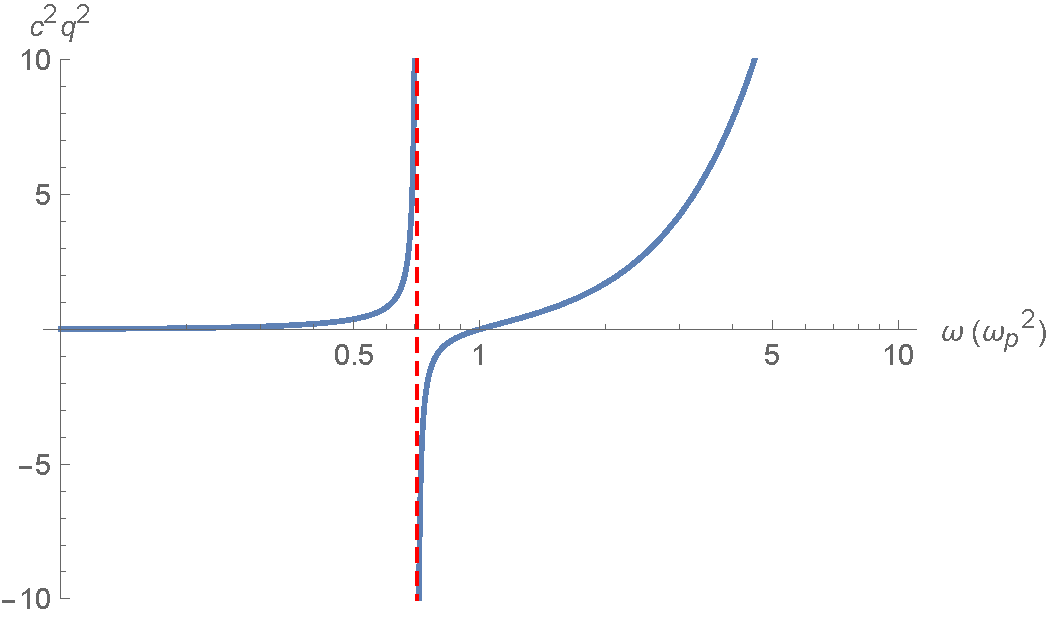
\includegraphics[width=\linewidth]{a&m_01_5b}
	\end{figure}
	
\end{multicols}

\subsubsection{The surface plasmon}
\textit{In the limit as } $qc \gg 1$, \textit{show that there is a solution at the frequency} $\omega = \omega_p / \sqrt{2}$. \textit{Show from an examination of K and K' that the wave is confined to the surface. Describe it's polarisation. This wave is known as a surface plasmon.}


\begin{multicols}{2}
	If $\omega = \omega_p / \sqrt{2}$, we can evaluate the original solution to determine the nature of the the wave and it's polarisation. Note what the limit $qc \gg \omega$ implies:
	\begin{align}
		q^2c^2 &\gg \omega^2\\
		\implies q^2c^2 = \omega ^2 \frac{\epsilon\left(\omega\right)}{\epsilon(\omega) +1 } &\gg \omega^2\\
		\to \frac{\epsilon(\omega)}{\epsilon(\omega) + 1} &\gg 1
	\end{align}
	
	Therefore as q is the coefficient for the speed of propagation in the x axis, the solution both in the vacuum and the metal oscillate fast relative to the frequency $\omega$. Evaluating $\epsilon(\omega)$: 
	\begin{align}
%		\epsilon\left(\frac{\omega_p}{\sqrt{2}}\right) &= 1 + \frac{4\pi}{\frac{\omega_p}{\sqrt{2}}}\left(\frac{1}{1-\imag \frac{\omega_p}{\sqrt{2}} \tau}\right)\left(\frac{ne^2\tau}{m_e}\right)\imag\\
%		&= 1 + \frac{\sqrt{2}}{{\omega_p}}\left(\frac{\sqrt{2}\tau}{\sqrt{2}-\imag \omega_p \tau}\right)\left(\omega_p^2\right)\imag\\
%		&= 1 + \frac{2\tau}{\sqrt{2}-\imag \omega_p \tau}\omega_p\imag
		\epsilon\left(\omega\right) &= 1 + \frac{4\pi}{\omega}\left(\frac{1}{1-\imag \omega \tau}\right)\left(\frac{ne^2\tau}{m_e}\right)\imag\\
		&= 1 + \frac{1}{\omega}\left(\frac{\tau}{1-\imag \omega \tau}\right)\left(\frac{4\pi ne^2}{m_e}\right)\imag\\
		&= 1 + \frac{1}{\omega}\left(\frac{\tau}{1-\imag \omega \tau}\right)\left(\omega_p^2\right)\imag\\
		&= 1 + \frac{\tau \omega_p^2}{\omega\left(1-\imag \omega \tau \right)}\imag\\
		&\nonumber\text{Multiply num. and den. by conjugate.}\\
		&= 1 + \frac{\tau \omega_p ^2}{\omega \left(1 + \omega^2 \tau^2\right)} \left(\imag - \omega \tau\right)\\
		&= 1 - \frac{\tau^2 \omega_p ^2}{1 + \omega^2 \tau^2} + \frac{\tau \omega_p ^2}{\omega \left(1 + \omega^2 \tau^2\right)}\imag\\
		&\nonumber\text{Still assuming conditions }\omega\tau \gg 1, \omega > \tau\\
		&\approx 1 - \frac{\omega_p^2}{\omega^2}
	\end{align}
	
	And evaluating q with $\omega \to \omega_p / \sqrt{2}$:
	\begin{align}
		q^2 &= \frac{\omega^2}{c^2} \frac{\epsilon(\omega)}{\epsilon(\omega)+1}\\
		q^2 &= \frac{\omega^2}{c^2} \left(\frac{1-\omega_p^2/\omega^2}{2 - \omega_p^2/\omega^2}\right)\\
		&= - \lim_{\omega\to \omega_p / \sqrt{2}} \left[\frac{\omega^2}{c^2 \left({2 - \omega_p^2/\omega^2}\right)}\right]\\
		q &= \pm \lim_{\omega\to \omega_p / \sqrt{2}} \left[\frac{\omega^2}{c \sqrt{2\omega - \omega_p^2}}\imag\right]\\
	\end{align}
	
		Considering K',
%	Evaluating q, K and K', we have:
%	
	\begin{align}
		K' &= \mp \frac{\omega}{c \sqrt{\epsilon(\omega) + 1}} \imag\\
		&= \mp \frac{\omega^2}{c\sqrt{2\omega^2 - \omega_p^2}}  \imag
	\end{align}
	Clearly the denominator diverges as $\omega \to \omega_p/\sqrt{2}$, implying that moving away from $z=0$ causes a large suppression in the plasmon amplitude.
	
	Considering K:
	\begin{align}
		K &= \pm \frac{\omega\epsilon(\omega)}{c \sqrt{\epsilon(\omega) + 1}} \imag\\
		&= \pm \frac{\omega^2}{c\sqrt{2\omega^2 - \omega_p^2}} \left(1 - \frac{\omega_p^2}{\omega^2}\right)  \imag\\
		&= \mp \lim_{\omega\to{\omega_p}/{\sqrt{2}}}\frac{\omega^2}{c\sqrt{2\omega^2 - \omega_p^2}} \imag\\
	\end{align}
	K has the same as the signed decay rate as K'. This is also the same as q. Therefore 
	\begin{align}
		\lim_{\omega\to\omega_p/\sqrt{2}} \left\{K' \approxeq K\right\} = q
	\end{align}
	Having confirmed the exponential components, consider the relation of coefficients between X and Z directions. A,B,C,D to check the polarisation. From part a), 
	\begin{align}
		\imag q A &= KB\\
		\imag q C &= -K'D
	\end{align}
	Using the relations for K, K' and q found above,
	\begin{align}
		\imag A &= B\\
		\imag C &= -D
	\end{align}
	This is the exact case of 90' phase between $E_x$ and $E_z$ components, meaning circularly polarised light.
\end{multicols}














